\chapter{A Lei n\textordmasculine 14.133}
\label{cap:14133}

As compras no setor público são, em geral, disciplinadas pelo Artigo 37 da Constituição Federal, que diz, em seu inciso XXI, que \emph{as obras, serviços, compras e alienações serão contratados mediante processo de licitação pública}.

Desde o dia 1{\textordmasculine} de abril de 2021, a lei que estabelece as normas para os processos licitatórios é a Lei n{\textordmasculine} 14.133, que agregou o conteúdo das leis n{\textordmasculine} 8.666 de 1993, lei anterior de licitações, n{\textordmasculine} 10.520 de 2002, lei que disciplinava os procedimentos para pregões e n{\textordmasculine} 12.462 de 2011, que disciplinava os procedimentos para a contratação de grandes obras principalmente no contexto das obras associadas à Copa do Mundo de 2014. No Estado de São Paulo, a lei 14.133 passou a vigorar desde o dia 1{\textordmasculine} de janeiro de 2024.

Além de agregar diversas leis que tratam de logística pública, a nova lei conta com diversas inovações. A primeira delas é o caráter completamente digital: todos os documentos que compõem a instrução processual de uma contratação tramitam nos Sistemas de Compras do Governo Federal\footnote{\url{https://www.gov.br/compras/pt-br}.} em formato digital. A interação entre os licitantes e os agentes de contratação também se dá por via digital. Ainda é possível realizar a fase de lances e negociação de forma presencial, mas a sessão pública deve ser gravada e disponibilizada\footnote{Artigo 17.}.

Outra inovação que talvez configure o aspecto mais importante é o foco na governança. O planejamento estratégico tornou-se obrigatório por meio do Plano de Contratações Anual (PCA) e tem por objetivo alinhar as contratações às leis orçamentárias, promovendo eficiência, efetividade e eficácia \citet{TCE2022}.

O ganho de governança se dá em diversos canais:
\begin{itemize}
    \item {combate às contratações ``emergenciais'' que deveriam ter sido planejadas;}
    \item {fim da fragmentação de contratações em múltiplas contratações elegíveis para dispensa por valor;}
    \item {separação de papéis entre o agente de contratação e o adjudicador, agora sendo a autoridade superior.}
\end{itemize}

A lei divide o processo de logística pública em três partes:
\begin{enumerate}
    \item{Planejamento da Contratação;}
    \item{Seleção do Fornecedor;}
    \item{Gestão do Contrato.}
\end{enumerate}

\begin{figure}
    \centering
    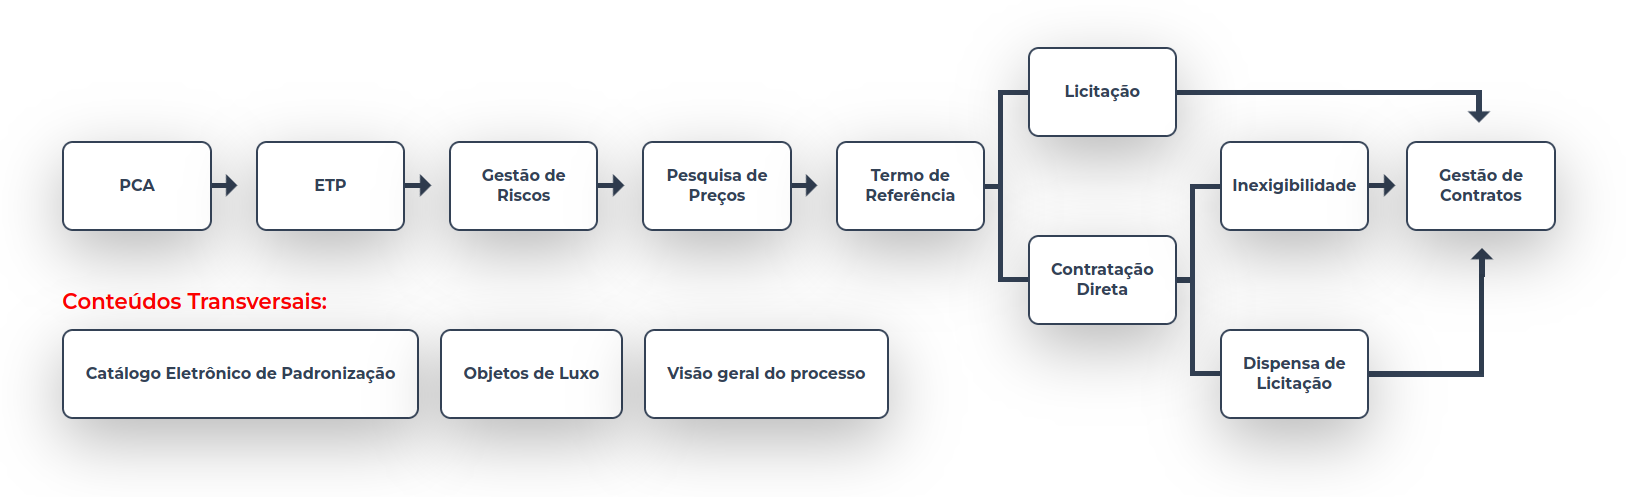
\includegraphics[scale=0.26]{conteudo/imagens/fluxo.png}
    \caption{Fluxo das Contratações. Fonte: https://compras.sp.gov.br/}
    \label{fig:fluxo}
\end{figure}

\section{Planejamento da Contratação}

A fase preparatória tem início com o registro das contratações planejadas para o próximo período, consolidando-se no Plano de Contratações Anual. Além de balizar quais serão as contratações esperadas para o próximo período, subsidiando a elaboração das leis orçamentárias, o plano de contratações será divulgado e mantido à disposição do público\footnote{Artigo 12.}. Isso possibilita tanto a otimização da logística pública por meio de contratações centralizadas quanto o conhecimento pelo mercado das demandas do setor público, fomentando o diálogo entre os demandantes e os ofertantes e abrindo espaço para a inovação.

O PCA deverá levar em conta tanto as aquisições ordinárias como papel, serviço de limpeza, suprimentos de informática etc, como as aquisições esporádicas que também fizerem parte do planejamento estratégico do órgão como a atualização do parque de computadores. \citet{TCE2022}

O locus que concentra a divulgação dos planos de contratação bem como as contratações propriamente ditas é o Portal Nacional de Contratações Públicas\footnote{\url{https://www.gov.br/pncp}.}. O fato de existir um local específico simplifica o acesso à demanda do setor público para os agentes do mercado.

A demanda que constitui o plano é formada de maneira mais abstrata quando da elaboração do PCA. A etapa que efetivamente caracteriza o objeto a ser contratado é o Estudo Técnico Preliminar (ETP).

O ETP tem por objetivo \emph{evidenciar o problema a ser resolvido e sua melhor solução, de modo a permitir a avaliação da viabilidade técnica e econômica da contratação}\footnote{Artigo 18.}, trata-se de um artefato que versa principalmente sobre a necessidade da contratação.

Os elementos obrigatórios em um ETP são a descrição da necessidade da contratação, a estimativa da quantidade, a \textbf{estimativa do valor}, justificativa para o parcelamento da solução e se a contratação é viável, ou não\footnote{Pode acontecer de a contratação não ser mais interessante no momento onde ela finalmente seria executada.}. É no ETP onde há a ligação entre o PCA e o objeto a ser contratado.

Descrita a necessidade, a próxima etapa consiste em verificar quais são os riscos associados à contratação. O exemplo mais imediato é ponderar sobre a situação onde o fornecedor não entrega o material.

Completando a trinca de artefatos, há o termo de referência. É o artefato responsável pelo enlace entre o cadastro de materiais e serviços do Governo Federal e o que se deseja contratar de fato. Esse enlace é realizado na seção das condições gerais dos objetos a serem contratados.

O termo de referência é onde está descrita a especificação técnica dos itens, inclusive, com previsão de marcas e modelos que serão aceitos\footnote{Vale ressaltar que a aquisição de bens de luxo é vedada. No Decreto n{\textordmasculine} 10.818 de 2017 há a menção sobre bens de luxo serem caracterizados como bens com alta elasticidade-renda, entretanto, não se especifica o que é ``alta''.} e, interessantemente, marcas e modelos que \textbf{não serão aceitos}. Em ambos os casos deve-se justificar.

Por fim, o termo de referência também versa sobre condições garantia e aspectos de gestão contratual como habilitação dos fornecedores, execução do objeto, pagamento e adequação orçamentária.

Todos os artefatos da fase preparatória tendem a melhorar a qualidade da informação disponível para todos os envolvidos.

\begin{figure}
    \centering
    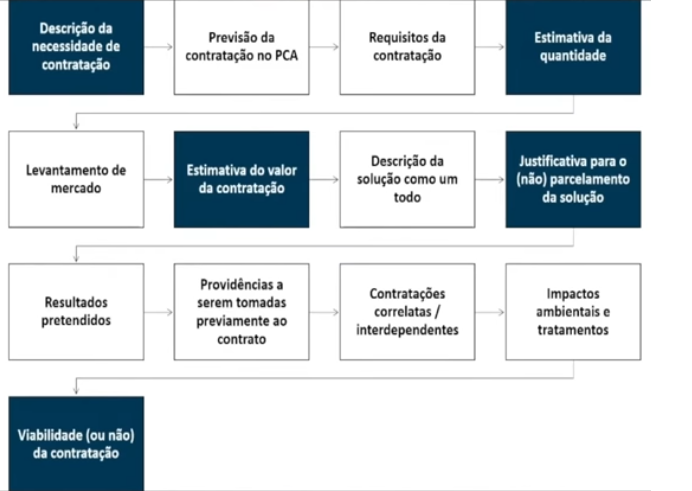
\includegraphics[scale=0.6]{conteudo/imagens/ETP.png}
    \caption{Elementos de um ETP. Os elementos obrigatórios estão nos quadrados com fundo azul. Fonte: https://www.youtube.com/watch?v=qlNwBv2MTxg.}
    \label{fig:ETP}
\end{figure}

\section{Seleção do Fornecedor}

A parte mais interessante para quem estuda mecanismos sem sombra de dúvidas é a que versa sobre a seleção de fornecedores. É nessa fase onde são empregradas as diversas modalidades bem como os instrumentos auxiliares com o intuito de realizar as contratações de bens ou serviços.

Existem dois modos de disputa: aberto e fechado. No modo aberto os licitantes apresentam suas propostas por meio de lances sucessivos. No modo fechado as propostas ficarão em sigilo até a data e hora designadas para a divulgação\footnote{Artigo 56.}.

A Lei n{\textordmasculine} 14.133 traz cinco modalidades:
\begin{enumerate}
    \item {pregão;}
    \item {concorrência;}
    \item {concurso;}
    \item {leilão;}
    \item {diálogo competitivo.}
\end{enumerate}

O pregão tende a ser a modalidade mais utilizada, pois é a modalidade obrigatória para bens e serviços comuns, inclusive de engenharia. O critério de julgamento é sempre \textbf{menor preço} ou \textbf{maior desconto}. Não é possível usar o modo fechado para o pregão, entretanto, é possível combinar ambos os modos.

A segunda modalidade mais utilizada é a concorrência \citet{TCE2023}. Trata-se da modalidade usada para obras, serviços de engenharia e serviços cuja descrição objetiva não é viável. A concorrência admite técnica e técnica e preço, além dos critérios de julgamento disponíveis para o pregão. É a única modalidade onde é possível selecionar fornecedores utilizando a técnica e preço como critério. Além disso, os critérios envolvendo técnica obrigam o uso do modo fechado. No caso de técnica e preço, a técnica pode corresponder por até 70\% da ponderação da pontuação\footnote{Artigo 36.}.

O concurso é a modalidade para a seleção de trabalho técnico, científico ou artístico cujo julgamento será necessariamente o de melhor técnica ou conteúdo artístico. O prêmio ou a remuneração do concurso são fixados já no edital de abertura do certame \citet{TCE2022}.

O leilão é a modalidade utilizada para a alienação de bens cujo critério de julgamento é o maior lance.

Por fim, o diálogo competitivo é uma inovação que prevê a divisão do certame em pelo menos duas fases. Na primeira fase o órgão público divulga a sua necessidade e os licitantes interessados submetem propostas para resolver a necessidade. Esse procedimento pode se repetir por diversas vezes. Findo o modelo, há a disputa onde só poderão participar os licitantes que fizeram parte das fases anteriores. Trata-se de uma modalidade cujo uso é restrito às contratações onde houver inovação tecnológica, impossibilidade de as especificações técnicas serem bem definidas pela Administração, impossibilidade de o órgão ter as necessidades satisfeitas com uma soluções disponíveis no mercado\footnote{Artigo 32.}.

No modo aberto é possível estabelecer via edital qual o intervalo mínimo entre os lances, embora não esteja explícito se isso será em moeda corrente ou em percentual. Ainda no modo aberto, uma vez que o vencedor tenha sido definido, é possível reiniciar a fase de lances com o objetivo de determinar a classificação de todos os licitantes.

Uma vez selecionado o vencedor, há a previsão de uma fase de negociação com o objetivo de melhorar as condições propostas. Se o preço final for superior ao preço de reserva, orçado no ETP, o licitante estará desclassificado e a negociação poderá ser realizada observando a classificação dos liciantes na etapa anterior.

Existem mais situações onde há a desclassificação de um licitante. São as seguintes:
\begin{itemize}
    \item {preço inexequível;}
    \item {inconformidade com as especificações técnicas;}
    \item {vícios \textbf{insanáveis} na proposta;}
    \item {preço final acima do preço de reserva.}
\end{itemize}

A situação de preço inexequível ocorre quando o preço final está muito abaixo do estimado. O licitante pode provar que tem condição de atender aos requisitos editalícios. Em obras de engenharia, por exemplo, é considerado inexequível um valor inferior a 75\% do orçado pela Administração\footnote{Artigo 59.}.

Há a preocupação em não desclassificar um licitante que tenha a possibilidade de sanar algum problema em sua proposta, potencialmente permitindo a participação de mais licitantes no certame. Como fato estilizado, vale dizer que existem atas processos licitatórios cuja desclassificação um licitante se deu pelo título da proposta não estar no formato solicitado no edital\footnote{\url{https://www.bec.sp.gov.br/bec_pregao_UI/Ata/becprp17001.aspx?qtQUXeWLUOPj5RlUGc8DXovFBgLp5CWxQKix0k9\%2FyGJsCit2rLDnEwsXtgEjFYna}}, diminuindo o número de concorrentes.

A Lei n{\textordmasculine} 14.133 prevê cinco procedimentos auxiliares para os processos licitatórios\footnote{Artigo 78.}. Quais sejam:
\begin{itemize}
    \item {credenciamento;}
    \item {pré-qualificação;}
    \item {procedimento de manifestação de interesse (PMI);}
    \item {registro cadastral;}
    \item {sistema de registro de preços.}
\end{itemize}

A pré-qualificação, o PMI e o registro cadastral são procedimentos que antecedem a licitação. O credenciamento e o sistema de registro de preços podem resultar na contratação de fornecedores, dispensando o procedimento licitatório \citet{TCE2022}.

O credenciamento pode ser realizado quando a contratação for paralela e não-excludente, isto é quando a contratação puder ser realizada de forma padronizada e simultânea. Quando não for possível a contratação imediata de todos os credenciados, deve ser adotado um critério de distribuição de demanda. Também é possível realizar o credenciamento quando há a situação de um mercado fluido, quando os valores variam constantemente de tal sorte que o procedimento licitatório regular se torna inviável\footnote{Artigo 79.}. Uma ocasião onde pode haver tal tipo de variação é em bens que estão sujeitos a variações cambiais \citet{TCE2022}.

A pré-qualificação é que almeja selecionar previamente bens e licitantes que atendam as exigências técnicas estabelecidas pela Administração\footnote{Artigo 80.} permitindo, posteriormente, a realização de um processo licitatório restrito aos bens e licitantes pré-qualificados. O cadastro de bens e licitantes deve ficar disponível para o público.

Tanto o credenciamento quanto a pré-qualificação são procedimentos que ficam permanentemente abertos para a inscrição de interessados.

O procedimento de manifestação de interesse é um chamamento público onde a Administração solicita à iniciativa privada a realização de estudos e propostas de soluções inovadoras para questões de relevância pública\footnote{Artigo 81.}. Ressalta-se que o PMI, diferente do diálogo competitivo, não obriga a realização de uma licitação posterior \citet{TCE2022}.

O registro cadastral é o cadastro de licitantes realizado no PNCP e atualizado anualmente. O cadastro classifica os inscritos em área de atuação, depois em categorias, segundo a qualificação técnica e econômico-financeira\footnote{Artigo 87.}.

\subsection{Sistema de Registro de Preços}
O sistema de registro de preços é definido como \emph{conjunto de procedimentos para realização, mediante contratação direta ou licitação nas modalidades pregão ou concorrência, de registro formal de preços relativos a prestação de serviços, a obras e a aquisição e locação de bens para contratações futuras}\footnote{Artigo 6.}.

O principal objetivo é evitar a realização de editais posteriores para a contratação de objetos de mesma categoria, adquirindo o que for efetivamente demandado no tempo em que houver tal demanda. O procedimento evita a aquisição desnecessária de bens bem como facilita a gestão de estoque.

Só é permitido como critério de julgamento menor preço ou maior desconto de tal sorte que o procedimento licitatório adotado geralmente será o pregão.

Podemos modelar a ata de registro de preços como um contrato onde são fornecidos o preço e a quantidade máxima de um determinado tipo de bem que \emph{pode} ser adquirido, funcionando como uma opção de compra. É possível a aquisição de \emph{zero} unidades, inclusive com a realização de outra licitação desde que devidamente justificada\footnote{Artigo 83.}.

Vale ressaltar que há algumas situações onde o preço pode ser diferente: quando o objeto for entregue em locais diferentes, em razão da forma e do local de acondicionamento, quando admitida a cotação variável em função do tamanho do lote e, finalmente, por razões justificadas no processo.

Existe a possibilidade de permitir que os licitantes registrem um quantitativo inferior ao previsto no edital bem como a possibilidade de se registrar mais de um fornecedor, desde que a cotação do objeto seja a mesma, assegurada a preferência de contratação de acordo com a ordem de classificação.

Por um lado, tal possibilidade é interessante, pois o perfil de custo marginal dos licitantes tipicamente não é constante, ao contrário do que acontece num contrato de registro de preços. Isso significa que se for vantajoso para um fornecedor entregar um quantitativo inferior ao solicitado, ele poderá participar do certame, aumentando potencialmente a competição. Por outro, há a possibilidade de divisão de lote, elevando o preço final\footnote{Basta que o primeiro colocado não oferte todo o quantitativo. Em vez de dar um lance para ganhar do segundo colocado, ele poderia dar um lance para ganhar apenas do terceiro colocado, majorando o lucro pela prática de um preço superior.}.

Uma inovação do sistema de registro de preços na nova lei versa sobre a possibilidade do registro de preço ser por grupo de itens desde que haja vantagem técnica ou econômica. Tal inovação ajuda a mitigar situações de exposição, onde há complementaridade entre bens, pois o caráter linear do registro de preços permite, em tese, quebrar essa sinergia\footnote{Um exemplo seria a aquisição de sapato por unidades de pé esquerdo e de pé direito. Um exemplo melhor seria a aquisição de peças de computador de uma mesma arquitetura.}.

Outra inovação versa sobre a participação de entidades não originalmente participantes, o que se convencionou a chamar de \emph{carona}. Quando da fase preparatória, há a obrigação de se realizar um procedimento público de intenção por, no mínimo, 8 dias para possibilitar a participação de outros órgãos na ata. Somente depois da adesão é que se calcula, de fato, o quantitativo.

Na nova lei há a possibilidade de adesão de órgãos que não participaram da fase preparatória e nem da fase de adesão desde que haja justificativa sobre a vantagem da adesão, a demonstração de que os valores registrados estão compatíveis com o mercado e a anuência do órgão gerenciador e do fornecedor. Contudo a adesão só pode realizada na direção do órgão mais restrito para o mais geral, isto é, órgãos federais não podem aderir a registros de preço estaduais e órgãos estaduais não podem aderir a registros de preço de órgãos municipais\footnote{Artigo 86.}.

Há duas limitações de quantitativo para a adesão de caronas nas atas de registro de preço: no máximo 50\% do quantitativo por carona e um limite global de duas vezes o quantitativo original para todos os caronas. A única exceção é caso se tratar de aquisição emergencial em ata gerenciada pelo Ministério da Saúde.

\begin{figure}
    \centering
    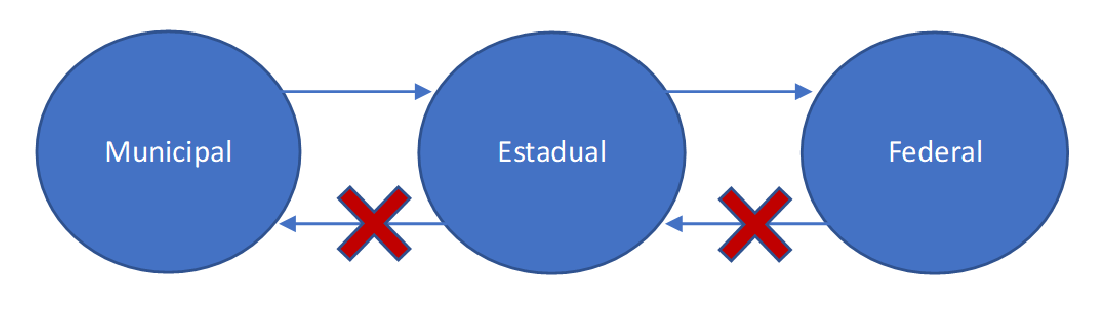
\includegraphics[scale=0.35]{conteudo/imagens/srp-adesao.png}
    \caption{A adesão não pode ser realizada de órgão mais geral para órgão mais restrito. Fonte: \citet{TCE2023}}
    \label{fig:srp-adesao}
\end{figure}

Na nova lei é possível haver registro de preço para serviços comuns de engenharia desde que exista projeto padronizado, sem complexidade técnica e operacional e que os serviços contratados sejam necessidade constante da Administração\footnote{Artigo 85.}. Um exemplo de serviço dessa natureza é a instalação de pontos de rede estruturada de dados. É um serviço padronizado, sem complexidade e demandado regularmente.